It has long been recognized that searchers prefer concise and specific answers, rather than lists of document results. In particular factoid questions, have been an active focus of research for decades due to both practical importance and relatively objective evaluation criteria.
As a particularly important example, a large proportion of Web search queries are looking for entities or their attributes \cite{Pound:2010:AOR:1772690.1772769}, a setting on which we focus in this work. 

Two relatively separate approaches for Question Answering (QA) have emerged: text-centric, or Text-QA and knowledge base-centric, or KBQA.
In the more traditional, Text-QA approach, systems used text document collections to retrieve passages relevant to a question and extract candidate answers \cite{dang2007overview}.
Unfortunately, an unstructured text passage does not provide explicit information about the candidate entities, which has to be inferred from the context.
The KBQA approach, which evolved from the database community, relies on large scale knowledge bases, such as dbPedia \cite{auer2007dbpedia}, Freebase \cite{Bollacker:2008:FCC:1376616.1376746} and WikiData \cite{Vrandecic:2014:WFC:2661061.2629489}, which store a vast amount of general knowledge about different kinds of entities.
This information, encoded as \texttt{[subject, predicate, object]} RDF triples, can be effectively queried using structured query languages, such as SPARQL.

Both approaches need to eventually deal with natural language questions, in which information needs are expressed by the vast majority of users.
While question understanding is difficult in itself, this setting is particularly challenging for KBQA systems, as it requires a translation of a text question into a structured query language.
That is challenging for a number of reasons, including the complexity of a KB schema, and many differences between natural language and knowledge representations. 
For example, Figure \ref{fig:example_sparql} gives a SPARQL query that retrieves the answer to a relatively simple question \textit{``who was the president of the Dominican Republic in 2010?''} from Freebase.

\begin{figure*}
\centering
% PREFIX : <http://rdf.freebase.com/ns/>
\begin{lstlisting}[frame=single,basicstyle=\small]
SELECT DISTINCT ?name {
   :m.027rn :government.governmental_jurisdiction.governing_officials ?gov_position .
   ?gov_position :government.government_position_held.basic_title :m.060c4 .
   ?gov_position :government.government_position_held.office_holder ?president .
   ?gov_position :government.government_position_held.from ?from_date .
   ?gov_position :government.government_position_held.to ?to_date .
   FILTER ( xsd:date(?from_date) <= "2010"^^xsd:date AND xsd:date(?to_date) >= "2010"^^xsd:date)
   ?president :type.object.name ?name
}
\end{lstlisting}
\caption{SPARQL query to retrieve the answer to the question \textit{``who was the president of the dominican republic in 2010?''}}
\label{fig:example_sparql}
\end{figure*}

Any KBQA systems must address three challenges, namely question entity identification to anchor the query process; candidate answer generation; and ranking.
We will show that these challenges can be alleviated by the appropriate use of external textual data.

The first problem that a KBQA system faces is question entity identification.
The performance of the whole system greatly depends on this stage \cite{yao-scratch-qa-naacl2015}, because it seeds the answer search process.
Question text is often quite short, may contain typos and other problems, that complicate entity linking.
Existing approaches are usually based on dictionaries that contain entity names, aliases and some other phrases, used to refer to the entities \cite{SPITKOVSKY12.266}.
These dictionaries are often noisy and incomplete, \eg to answer the question \textit{``what year did tut became king?''} a system needs to detect a mention \textit{``tut''}, which refers to the entity \texttt{Tutankhamun}.
If a dictionary doesn't contain a mapping \textit{``tut''} $\rightarrow$ \texttt{Tutankhamun}, as happens for one of the state of the art systems, a system will not be able to answer the question correctly.
Such less popular name variations are often used along with full names inside text documents, for example, to avoid repetitions.
Therefore, we propose to look into web search results to find variations of question entity names, which can be easier to link to a KB (Figure \ref{fig:web_search_entitylink}).
This idea has been shown effective in entity linking for web search queries\footnote{http://web-ngram.research.microsoft.com/ERD2014/} \cite{SMAPH_ERD:2014}.
% Figure \ref{fig:web_search_entitylink} presents web search results for the query \textit{``what year did tut became king?''}, which shows that indeed many documents mention the full name of the entity.

\begin{figure}[!h]
\centering
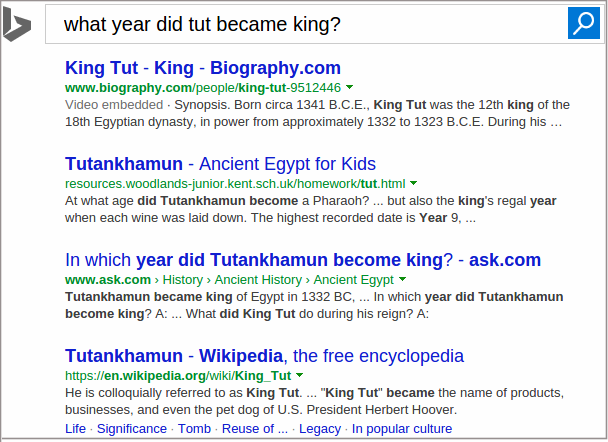
\includegraphics[width=0.45\textwidth]{img/web_search_entitylink}
\caption{Search results for the question \textit{``what year did tut became king?''}, which mention both the full name of the king and the correct answer to the question}
\label{fig:web_search_entitylink}
\end{figure}

After question entities have been identified, answer candidates need to be generated and ranked to select the best answer.
A candidate query includes one or multiple triple patterns with predicates, corresponding to words and phrases in the question.
Existing knowledge base question answering approaches \cite{ACCU:2015,Berant:EMNLP13,berant2014semantic,berant2015imitation,BordesCW14:emnlp,yao2014freebase} rely on a lexicon, learned from manually labeled training data, and supported by additional resources, such as question paraphrases \cite{berant2014semantic} and weakly labeled sentences from a large text collection \cite{yao2014information}.
Such training data tends to be small compared to the number of different predicates in a KB, and therefore the coverage of these lexicons is limited.
By our estimate, in a popular WebQuestions KBQA dataset, the answers to $\sim$5.5\% of test questions (112 out of 2032) involve a predicate that does not appear as a ground truth in the training set.
For example, an RDF triple \texttt{[Bigos, food.dish.type\_of\_dish1, Stew]} answers the question \textit{``what are bigos?''}, but no other examples in the training set involve this predicate.
In addition, a lexicon needs to cover all different ways a predicate can be asked about.
For example, questions \textit{``who did jon gosselin cheat with?''} and \textit{``who is the woman that john edwards had an affair with?''} are answered by the same KB predicate, but use different language.
Therefore, presence of the first question in a training set might not help to answer the later one.
On the other hand, traditional Text-QA systems benefit from the redundancy of the information on the Web, where the same facts are stated multiple times in many different ways \cite{Lin:2007:EPU:1229179.1229180}.
This increases the chances of a good lexical match between a question and answer statements, which makes even some relatively simple counting-based techniques quite effective \cite{brill2002analysis}.
We propose to adapt these ideas from text-based question answering for KBQA.
The right part of the Figure \ref{fig:model} shows web search results, a community question answering page, and text fragments mentioning pairs of entities, that can be useful to answer the question about John Edwards' affair.

To summarize, our contributions are three-fold:
\begin{itemize}
\item A novel ``hybrid'' knowledge base question answering system, which uses both structured data from a knowledge base and unstructured text resources. Section \ref{section:method} describes the architecture of our system, and Section \ref{section:eval} shows that this fusion improves the performance of a state of the art KBQA system.
\item Novel data sources and techniques for KBQA: enhancing question entity identification by analyzing web search results (Section \ref{section:method:web}); improving predicate matching by mining CQA data (Section \ref{section:method:cqa}); and improving candidate ranking by incorporating text-corpus statistics (Section \ref{section:method:clueweb}).
\item Comprehensive empirical analysis of our system on a popular WebQuestions benchmark, demonstrating that using additional text resources can improve the performance of a state-of-the-art KBQA system (Section \ref{section:eval}). In addition, we conduct an extensive analysis of the system to identify promising directions for future improvements (Section \ref{section:analysis}).
\end{itemize}

Taken together, this work introduces a number of techniques of using external text that significantly improve the performance of the KBQA approach.
More broadly, our work bridges the gap between Text-QA and KBQA worlds, demonstrating an important step forward towards combining unstructured and structured data for question answering.


% -------------------------------------------

%There are many problems in KBQA:
%\begin{itemize}
%\item lexical variations, we can call the same thing in million ways
%\item representation variation - similar data can be represented in multiple ways, e.g. capital of the state in Australia location.australian\_state.capital\_city, while in the US you will have totally different predicate. HOWEVER, these are old predicate and marked deprecated. There is another predicate that should be the same for both cases.
%\item Incomplete, some data is simply missing or details are not present. E.g. who is the woman that john edwards had an affair with?, there is a triple that says that he had sexual relationships with Rielle Hunter, but there is no details...
%\item Related to the previous - many predicates are simply not present. There is something related, but not exactly what is asked about. Example: where did andy murray started playing tennis? We can find the answer entity, but the triple won't say that he started playing there.
%\end{itemize}

%In \cite{Sun:2015:ODQ:2736277.2741651} authors report pretty low score for Sempre on TREC and Bing QA datasets.

% Questions and corresponding answers are often expressed differently and researchers in question answering studied different ways to bridge this lexical gap, \eg using translation models \cite{Murdock:2005:TMS:1220575.1220661} and distributional semantics \cite{yu2014deep}.


